% This file was created with tikzplotlib v0.10.1.
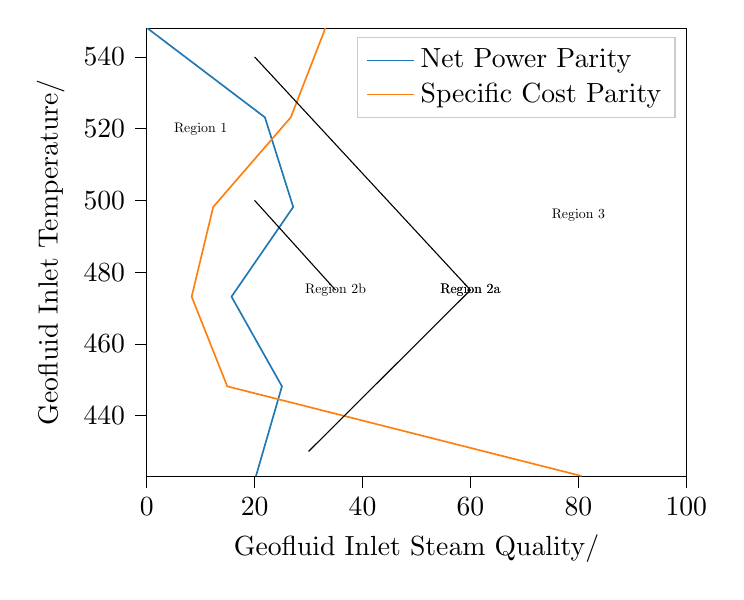
\begin{tikzpicture}

\definecolor{darkgray176}{RGB}{176,176,176}
\definecolor{darkorange25512714}{RGB}{255,127,14}
\definecolor{lightgray204}{RGB}{204,204,204}
\definecolor{steelblue31119180}{RGB}{31,119,180}

\begin{axis}[
legend cell align={left},
legend style={fill opacity=0.8, draw opacity=1, text opacity=1, draw=lightgray204},
tick align=outside,
tick pos=left,
x grid style={darkgray176},
xlabel={Geofluid Inlet Steam Quality/\unit{\percent}},
xmin=0, xmax=100,
xtick style={color=black},
y grid style={darkgray176},
ylabel={Geofluid Inlet Temperature/\unit{\K}},
ymin=423, ymax=548,
ytick style={color=black}
]
\addplot [semithick, steelblue31119180]
table {%
20.2574810001872 423.15
25.0672234506447 448.15
15.7209666111048 473.15
27.155997056422 498.15
21.9106672040425 523.15
0 548.15
};
\addlegendentry{Net Power Parity}
\addplot [semithick, darkorange25512714]
table {%
80.5840390695152 423.15
14.9367985901707 448.15
8.33516703959791 473.15
12.3239556472682 498.15
26.7033895623133 523.15
33.1523929813526 548.15
};
\addlegendentry{Specific Cost Parity}
\draw (axis cs:10,520) node[
  scale=0.5,
  text=black,
  rotate=0.0
]{Region 1};
\draw[-,draw=black] (axis cs:60,475) -- (axis cs:20,540);
\draw (axis cs:60,475) node[
  scale=0.5,
  text=black,
  rotate=0.0
]{Region 2a};
\draw[-,draw=black] (axis cs:60,475) -- (axis cs:30,430);
\draw (axis cs:60,475) node[
  scale=0.5,
  text=black,
  rotate=0.0
]{Region 2a};
\draw[-,draw=black] (axis cs:35,475) -- (axis cs:20,500);
\draw (axis cs:35,475) node[
  scale=0.5,
  text=black,
  rotate=0.0
]{Region 2b};
\draw (axis cs:80,495) node[
  scale=0.5,
  anchor=base,
  text=black,
  rotate=0.0
]{Region 3};
\end{axis}

\end{tikzpicture}
